% !TEX root = ../notes_unsupervisedlearning.tex
% Chapter 4: Density and Graph-Based Clustering
%%%%%%%%%%%%%%%%%%%%%%%%%%%%%%%%%%%%%%%%%%%%%%%%%%%%%%%%%%%%%%%%%%%%%%

\chapter{Density and Graph-Based Clustering}\index{DBSCAN}\index{Spectral Clustering}
\newthought{Structure is connectivity, not just proximity.}

%═══════════════════════════════════════════════════════════════════════
% BLOCK 1: INTRODUCTION
%═══════════════════════════════════════════════════════════════════════

\section{The Why}

\marginnote{Real-world clusters are often non-spherical: rivers, roads, social networks.}

K-Means and hierarchical clustering assume clusters are defined by distance to centers or pairwise distances. But many real datasets have:
\begin{itemize}
    \item \textbf{Arbitrary shapes}: Clusters that are elongated, curved, or non-convex
    \item \textbf{Noise}: Points that don't belong to any cluster
    \item \textbf{Varying densities}: Some regions denser than others
\end{itemize}

Consider GPS trajectories of taxis: clusters are road networks, not spheres. Or social networks: communities are defined by connections, not geometric distance.

\textbf{Density-based clustering} defines clusters as dense regions separated by sparse regions. \textbf{Graph-based clustering} finds clusters as connected components or communities in a similarity graph.

\subsection{Hands-On Experience}

\begin{marginfigure}
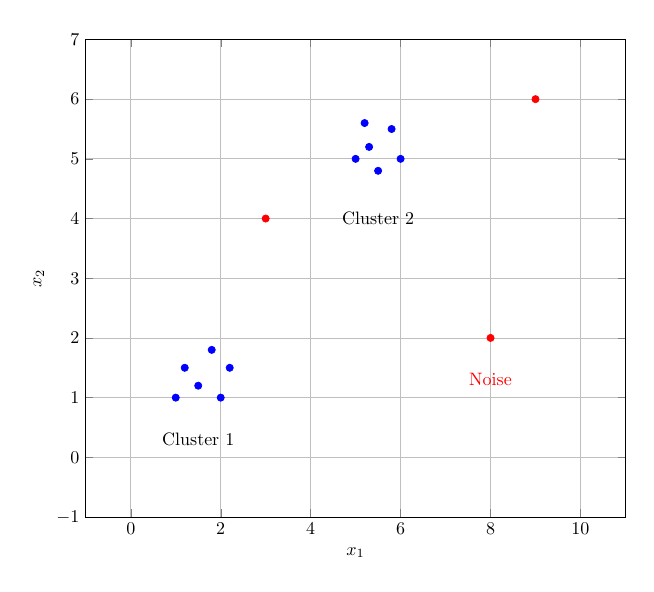
\begin{tikzpicture}[scale=0.65]
    \begin{axis}[
        xlabel={$x_1$},
        ylabel={$x_2$},
        xmin=-1, xmax=11,
        ymin=-1, ymax=7,
        width=\textwidth,
        height=0.9\textwidth,
        grid=major,
    ]
    % Dense cluster 1
    \addplot[only marks, mark=*, mark size=2pt, blue] coordinates {
        (1,1) (1.2,1.5) (1.5,1.2) (2,1) (1.8,1.8) (2.2,1.5)
    };
    % Dense cluster 2
    \addplot[only marks, mark=*, mark size=2pt, blue] coordinates {
        (5,5) (5.3,5.2) (5.5,4.8) (5.8,5.5) (6,5) (5.2,5.6)
    };
    % Noise points
    \addplot[only marks, mark=*, mark size=2pt, red] coordinates {
        (8,2) (3,4) (9,6)
    };
    % Labels
    \node at (axis cs:1.5,0.3) {Cluster 1};
    \node at (axis cs:5.5,4) {Cluster 2};
    \node[red] at (axis cs:8,1.3) {Noise};
    \end{axis}
\end{tikzpicture}
\caption{Two dense clusters and three noise points.}
\end{marginfigure}

Given the points shown, answer:
\begin{enumerate}
    \item Which points are in "dense" regions? (Say, $\geq 3$ neighbors within distance 1)
    \item Which points might be "noise"?
    \item Can K-Means correctly identify the noise points?
\end{enumerate}

Density-based methods naturally identify the isolated points as noise while grouping the dense regions as clusters.

\subsection{Learning Objectives}

After this lecture, you will be able to:
\begin{enumerate}
    \item Implement DBSCAN and explain its parameters ($\varepsilon$, minPts)
    \item Distinguish core, border, and noise points
    \item Apply OPTICS for multi-density datasets
    \item Construct and interpret spectral clustering
    \item Choose appropriate density/graph methods based on data characteristics
\end{enumerate}

%═══════════════════════════════════════════════════════════════════════
% BLOCK 2: MAIN THEORY
%═══════════════════════════════════════════════════════════════════════

\section{DBSCAN}

\marginnote{DBSCAN: Density-Based Spatial Clustering of Applications with Noise (Ester et al., 1996)}

\subsection{Core Concepts}

DBSCAN defines clusters based on \textbf{density reachability}. Key parameters:
\begin{itemize}
    \item $\varepsilon$ (eps): Neighborhood radius
    \item minPts: Minimum points to form a dense region
\end{itemize}

\begin{definition}[$\varepsilon$-neighborhood]
The $\varepsilon$-neighborhood of point $p$ is:
\begin{equation}
    N_\varepsilon(p) = \{q \in X : d(p, q) \leq \varepsilon\}
\end{equation}
\end{definition}

\begin{definition}[Point types]
\begin{itemize}
    \item \textbf{Core point}: $|N_\varepsilon(p)| \geq \text{minPts}$
    \item \textbf{Border point}: Not core, but in $N_\varepsilon$ of a core point
    \item \textbf{Noise point}: Neither core nor border
\end{itemize}
\end{definition}

\begin{figure}[h]
\centering
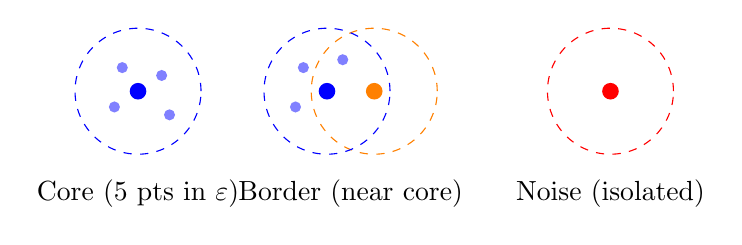
\begin{tikzpicture}[scale=1.0]
    % Core point
    \fill[blue] (0,0) circle (3pt);
    \draw[blue, dashed] (0,0) circle (0.8cm);
    \fill[blue!50] (0.3,0.2) circle (2pt);
    \fill[blue!50] (-0.2,0.3) circle (2pt);
    \fill[blue!50] (0.4,-0.3) circle (2pt);
    \fill[blue!50] (-0.3,-0.2) circle (2pt);
    \node[anchor=north] at (0,-1) {Core (5 pts in $\varepsilon$)};

    % Border point
    \fill[orange] (3,0) circle (3pt);
    \draw[orange, dashed] (3,0) circle (0.8cm);
    \fill[blue] (2.4,0) circle (3pt);
    \draw[blue, dashed] (2.4,0) circle (0.8cm);
    \fill[blue!50] (2.1,0.3) circle (2pt);
    \fill[blue!50] (2.0,-0.2) circle (2pt);
    \fill[blue!50] (2.6,0.4) circle (2pt);
    \node[anchor=north] at (2.7,-1) {Border (near core)};

    % Noise point
    \fill[red] (6,0) circle (3pt);
    \draw[red, dashed] (6,0) circle (0.8cm);
    \node[anchor=north] at (6,-1) {Noise (isolated)};
\end{tikzpicture}
\caption{DBSCAN point classification with minPts=4. Core points have enough neighbors; border points are near cores; noise points are isolated.}
\end{figure}

\begin{definition}[Density reachability]
Point $q$ is \textbf{directly density-reachable} from $p$ if:
\begin{enumerate}
    \item $p$ is a core point
    \item $q \in N_\varepsilon(p)$
\end{enumerate}
Point $q$ is \textbf{density-reachable} from $p$ if there exists a chain $p = p_1, p_2, \ldots, p_n = q$ where each $p_{i+1}$ is directly density-reachable from $p_i$.
\end{definition}

\marginnote{Density-reachability is not symmetric: a border point is reachable from a core, but not vice versa.}

\subsection{The Algorithm}

\begin{algorithm}[H]
\caption{DBSCAN}
\begin{algorithmic}[1]
\Require Data $X$, parameters $\varepsilon$, minPts
\Ensure Cluster labels for each point
\State Mark all points as unvisited
\State $C \gets 0$ \Comment{Cluster counter}
\For{each unvisited point $p$}
    \State Mark $p$ as visited
    \State $N \gets N_\varepsilon(p)$
    \If{$|N| < \text{minPts}$}
        \State Mark $p$ as noise (may change later)
    \Else
        \State $C \gets C + 1$
        \State \Call{ExpandCluster}{$p, N, C, \varepsilon, \text{minPts}$}
    \EndIf
\EndFor
\end{algorithmic}
\end{algorithm}

\begin{algorithm}[H]
\caption{ExpandCluster}
\begin{algorithmic}[1]
\Procedure{ExpandCluster}{$p, N, C, \varepsilon, \text{minPts}$}
    \State Add $p$ to cluster $C$
    \For{each point $q$ in $N$}
        \If{$q$ is unvisited}
            \State Mark $q$ as visited
            \State $N' \gets N_\varepsilon(q)$
            \If{$|N'| \geq \text{minPts}$}
                \State $N \gets N \cup N'$
            \EndIf
        \EndIf
        \If{$q$ is not yet in any cluster}
            \State Add $q$ to cluster $C$
        \EndIf
    \EndFor
\EndProcedure
\end{algorithmic}
\end{algorithm}

\subsection{Parameter Selection}

\marginnote{The k-distance plot helps choose $\varepsilon$.}

Choosing $\varepsilon$ and minPts:
\begin{itemize}
    \item \textbf{minPts}: Rule of thumb: $\geq d + 1$ where $d$ is dimensionality. Common: minPts $= 4$ or $5$.
    \item \textbf{$\varepsilon$}: Plot the $k$-distance (distance to $k$-th nearest neighbor) sorted. Look for an "elbow."
\end{itemize}

\begin{marginfigure}
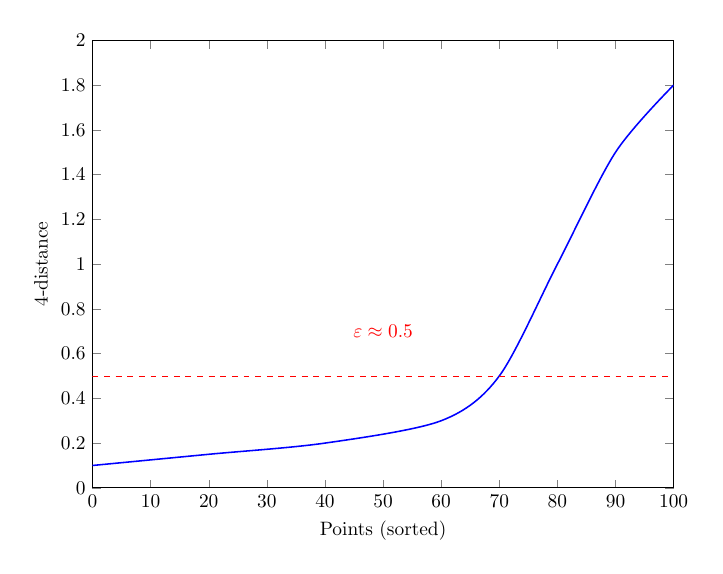
\begin{tikzpicture}[scale=0.7]
    \begin{axis}[
        xlabel={Points (sorted)},
        ylabel={4-distance},
        xmin=0, xmax=100,
        ymin=0, ymax=2,
        width=\textwidth,
        height=0.8\textwidth,
    ]
    \addplot[blue, thick, smooth] coordinates {
        (0,0.1) (20,0.15) (40,0.2) (60,0.3) (70,0.5) (80,1.0) (90,1.5) (100,1.8)
    };
    \draw[red, dashed] (axis cs:0,0.5) -- (axis cs:100,0.5);
    \node[red] at (axis cs:50,0.7) {$\varepsilon \approx 0.5$};
    \end{axis}
\end{tikzpicture}
\caption{k-distance plot. The elbow suggests $\varepsilon \approx 0.5$.}
\end{marginfigure}

\textbf{Complexity}: $O(n^2)$ naive, $O(n \log n)$ with spatial indexing (k-d tree, ball tree).


\section{OPTICS}

\marginnote{OPTICS: Ordering Points To Identify the Clustering Structure}

DBSCAN struggles with clusters of varying density. \textbf{OPTICS} addresses this by producing a \textbf{reachability plot} instead of a fixed clustering.

\begin{definition}[Reachability distance]
\begin{equation}
    \text{reach-dist}(p, o) = \max(\text{core-dist}(o), d(o, p))
\end{equation}
where core-dist($o$) is the distance to the minPts-th nearest neighbor.
\end{definition}

OPTICS orders points such that nearby points (in terms of density) are adjacent, then plots reachability distance vs. ordering. Valleys in the plot indicate clusters.

\begin{figure}[h]
\centering
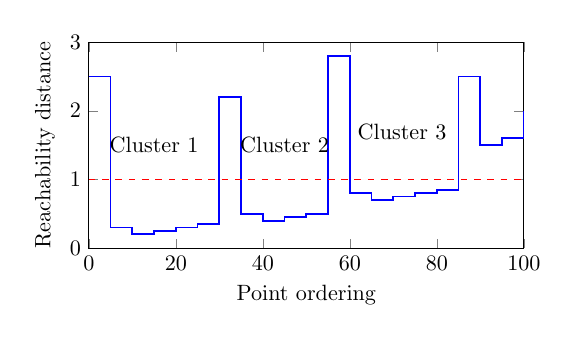
\begin{tikzpicture}[scale=0.8]
    \begin{axis}[
        xlabel={Point ordering},
        ylabel={Reachability distance},
        xmin=0, xmax=100,
        ymin=0, ymax=3,
        width=0.7\textwidth,
        height=0.4\textwidth,
    ]
    \addplot[blue, thick, const plot] coordinates {
        (0,2.5) (5,0.3) (10,0.2) (15,0.25) (20,0.3) (25,0.35)
        (30,2.2) (35,0.5) (40,0.4) (45,0.45) (50,0.5)
        (55,2.8) (60,0.8) (65,0.7) (70,0.75) (75,0.8) (80,0.85)
        (85,2.5) (90,1.5) (95,1.6) (100,2.0)
    };
    \draw[red, dashed] (axis cs:0,1.0) -- (axis cs:100,1.0);
    \node at (axis cs:15,1.5) {Cluster 1};
    \node at (axis cs:45,1.5) {Cluster 2};
    \node at (axis cs:72,1.7) {Cluster 3};
    \end{axis}
\end{tikzpicture}
\caption{OPTICS reachability plot. Valleys indicate dense clusters; peaks indicate sparse separations.}
\end{figure}

Cutting the reachability plot at different thresholds gives different clusterings, similar to cutting a dendrogram.


\section{Mean Shift}

\marginnote{Mean Shift finds modes of the density function.}

\textbf{Mean Shift} is a mode-seeking algorithm:

\begin{algorithm}[H]
\caption{Mean Shift}
\begin{algorithmic}[1]
\For{each point $x$}
    \Repeat
        \State $m(x) \gets \frac{\sum_{x_i \in N_h(x)} K(x_i - x) \cdot x_i}{\sum_{x_i \in N_h(x)} K(x_i - x)}$
        \State $x \gets m(x)$
    \Until{convergence}
\EndFor
\State Cluster points that converge to the same mode
\end{algorithmic}
\end{algorithm}

where $K$ is a kernel (e.g., Gaussian) and $h$ is the bandwidth.

\textbf{Properties}:
\begin{itemize}
    \item Automatically finds number of clusters
    \item Can find non-convex clusters
    \item Bandwidth $h$ is the key parameter
\end{itemize}


\section{Spectral Clustering}

\marginnote{Spectral clustering uses the graph Laplacian to find clusters.}

\textbf{Spectral clustering} transforms clustering into a graph partitioning problem:

\subsection{Algorithm Overview}

\begin{enumerate}
    \item \textbf{Build similarity graph}: $W_{ij} = \exp(-\|x_i - x_j\|^2 / 2\sigma^2)$
    \item \textbf{Compute Laplacian}: $L = D - W$ where $D_{ii} = \sum_j W_{ij}$
    \item \textbf{Find eigenvectors}: Compute $k$ smallest eigenvectors of $L$
    \item \textbf{Cluster}: Run K-Means on the eigenvector embedding
\end{enumerate}

\begin{figure}[h]
\centering
\begin{tikzpicture}[scale=0.65]
    % Original space
    \begin{axis}[
        name=orig,
        title={Original space},
        xlabel={$x_1$}, ylabel={$x_2$},
        xmin=-3, xmax=3, ymin=-3, ymax=3,
        width=0.4\textwidth,
        axis equal,
    ]
    % Two moons
    \addplot[only marks, mark=*, mark size=1.5pt, blue, domain=0:180, samples=25]
        ({cos(x)}, {sin(x)});
    \addplot[only marks, mark=*, mark size=1.5pt, red, domain=0:180, samples=25]
        ({1+cos(x)}, {0.5-sin(x)});
    \end{axis}

    % Arrow
    \node at (4.5,1.5) {$\xrightarrow{\text{Spectral}}$};

    % Spectral space
    \begin{axis}[
        at={(orig.east)}, anchor=west, xshift=2.5cm,
        title={Spectral embedding},
        xlabel={$v_1$}, ylabel={$v_2$},
        xmin=-0.3, xmax=0.3, ymin=-0.3, ymax=0.3,
        width=0.4\textwidth,
        axis equal,
    ]
    \addplot[only marks, mark=*, mark size=1.5pt, blue] coordinates {
        (-0.15,0.1) (-0.14,0.08) (-0.13,0.09) (-0.12,0.07)
        (-0.16,0.11) (-0.17,0.09) (-0.11,0.08)
    };
    \addplot[only marks, mark=*, mark size=1.5pt, red] coordinates {
        (0.15,-0.1) (0.14,-0.08) (0.13,-0.09) (0.12,-0.07)
        (0.16,-0.11) (0.17,-0.09) (0.11,-0.08)
    };
    \end{axis}
\end{tikzpicture}
\caption{Spectral clustering separates non-convex clusters by embedding into eigenvector space.}
\end{figure}

\subsection{Graph Laplacian}

The \textbf{unnormalized Laplacian}:
\begin{equation}
    L = D - W
\end{equation}

The \textbf{normalized Laplacian}:
\begin{equation}
    L_{\text{sym}} = D^{-1/2} L D^{-1/2} = I - D^{-1/2} W D^{-1/2}
\end{equation}

\marginnote{The number of zero eigenvalues equals the number of connected components.}

Key property: The eigenvectors of $L$ encode cluster structure. The smallest eigenvalue is always 0 (with eigenvector $\mathbf{1}$). The second-smallest eigenvector (Fiedler vector) partitions the graph.


\section{Community Detection}

\marginnote{Modularity measures how "modular" a network partition is.}

For networks/graphs, \textbf{community detection} finds groups of densely connected nodes. \textbf{Modularity}:
\begin{equation}
    Q = \frac{1}{2m} \sum_{ij} \left[ A_{ij} - \frac{k_i k_j}{2m} \right] \delta(c_i, c_j)
\end{equation}
where $A$ is the adjacency matrix, $k_i$ is the degree of node $i$, $m$ is total edges, and $c_i$ is the community of node $i$.

The \textbf{Louvain algorithm} greedily optimizes modularity:
\begin{enumerate}
    \item Assign each node to its own community
    \item Move nodes to neighboring communities to maximize modularity
    \item Aggregate communities into super-nodes
    \item Repeat until no improvement
\end{enumerate}


%═══════════════════════════════════════════════════════════════════════
% BLOCK 3: STUDENT ACTIVATION
%═══════════════════════════════════════════════════════════════════════

\section{Examples \& Exercises}

\subsection{Exercise 1: DBSCAN by Hand}

Given points: $(0,0), (1,0), (1,1), (0,1), (5,5), (10,10)$

With $\varepsilon = 1.5$ and minPts $= 3$:
\begin{enumerate}
    \item Classify each point as core, border, or noise
    \item Identify the clusters
\end{enumerate}

\textbf{Solution}:
\begin{itemize}
    \item $(0,0)$: Neighbors within 1.5: $(1,0), (0,1)$. Count = 3 (including self). Core.
    \item $(1,0)$: Neighbors: $(0,0), (1,1)$. Count = 3. Core.
    \item $(1,1)$: Neighbors: $(1,0), (0,1)$. Count = 3. Core.
    \item $(0,1)$: Neighbors: $(0,0), (1,1)$. Count = 3. Core.
    \item $(5,5)$: No neighbors within 1.5. Noise.
    \item $(10,10)$: No neighbors within 1.5. Noise.
\end{itemize}
Cluster 1: $\{(0,0), (1,0), (1,1), (0,1)\}$. Noise: $\{(5,5), (10,10)\}$.

\subsection{Exercise 2: Parameter Sensitivity}

How would the clustering change if:
\begin{enumerate}
    \item $\varepsilon = 0.5$ (smaller)?
    \item minPts $= 5$ (larger)?
\end{enumerate}

\textbf{Solution}:
\begin{enumerate}
    \item With $\varepsilon = 0.5$: Most points become noise (neighbors too far).
    \item With minPts $= 5$: All points become noise (no point has 5 neighbors within $\varepsilon=1.5$).
\end{enumerate}

\subsection{Exercise 3: Spectral vs K-Means}

Why does K-Means fail on concentric circles while spectral clustering succeeds?

\textbf{Solution}: K-Means assigns points to nearest centroid, which cannot separate concentric circles (centroids would be at the center). Spectral clustering builds a graph where inner circle points connect to each other (not to outer circle), then the graph Laplacian eigenvectors separate them.


\section{Self-Reflection \& Recap}

\subsection{Reflection Questions}
\begin{enumerate}
    \item Why can DBSCAN find clusters of arbitrary shape while K-Means cannot?
    \begin{quote}
        \textit{DBSCAN defines clusters via density-connectivity: any shape can emerge from chains of core points. K-Means assigns to nearest centroid, implicitly assuming convex Voronoi regions.}
    \end{quote}

    \item How do you choose $\varepsilon$ and minPts in practice?
    \begin{quote}
        \textit{Use the k-distance plot to find $\varepsilon$ (the elbow), and set minPts $\geq d+1$ where $d$ is dimensionality. Validate by inspecting results.}
    \end{quote}

    \item What is the intuition behind spectral clustering's use of eigenvectors?
    \begin{quote}
        \textit{The graph Laplacian's eigenvectors encode how to partition the graph with minimal edge cuts. Points in the same cluster have similar eigenvector values, so K-Means in this space finds good partitions.}
    \end{quote}
\end{enumerate}

\subsection{Key Concepts}
\begin{itemize}
    \item \textbf{Density-based methods} define clusters as dense regions separated by sparse regions
    \item \textbf{DBSCAN} naturally handles noise and arbitrary shapes
    \item \textbf{OPTICS} extends DBSCAN to varying densities via reachability plots
    \item \textbf{Spectral clustering} uses graph structure to find non-convex clusters
    \item \textbf{Parameter selection} ($\varepsilon$, bandwidth, number of neighbors) is critical
\end{itemize}

\subsection{Next Chapter Teaser}
\marginnote{Teaser: From clustering to compression}
\newthought{We've learned to find structure through clustering.} But high-dimensional data is hard to cluster, visualize, and process. What if we could compress data while preserving its essential structure? The next chapter explores \textbf{dimensionality reduction}---from classical PCA to modern t-SNE and UMAP.
